\section{Digression on Self-Similar Fractals}

In this chapter, we demonstrate a geometric application of the contraction
mapping theorem. We will consider a metric space whose points are geometric
figures and will see that self-similar fractals are nothing but fixed points of
suitable contractive maps.

\begin{definition}
Let $A$ and $B$ be non-empty subsets of $\RR^n$. We define the \emph{Hausdorff
distance}
\mymargin{Hausdorff distance}
\index{distance!Hausdorff}
between $A$ and $B$ as:
\[
    d_{\H}(A,B) = \max\ENCLOSE{\sup_{a\in A}\inf_{b\in B} \abs{a-b}, \sup_{b\in
  B} \inf_{a\in A} \abs{a-b}}.
\]

We define
\[
 \K(\RR^n) = \ENCLOSE{A \subset \RR^n \colon \text{$A$ closed, bounded, non-empty}}.
\]
\end{definition}

\begin{theorem}[characterization of the Hausdorff distance]
If $A$ and $B$ are compact subsets of $\RR^n$ (i.e., closed and bounded), then
for every $r \in \RR$, we have
\[
  d_\H(A,B) \le r
\]
if and only if both of the following properties hold:
\begin{enumerate}
\item for every $a\in A$ there exists $b\in B$ such that $\abs{a-b}\le r$;
\item for every $b\in B$ there exists $a\in A$ such that $\abs{a-b}\le r$.
\end{enumerate}
\end{theorem}
%
\begin{proof}
For every non-empty compact set $A$ and for every $x\in \RR^n$, we define the
distance between the point $x$ and the set $A$ as:
\[
  d(x,A) = \min_{a\in A} \abs{x-a}.
\]
The minimum exists because $A$ is compact and $a\mapsto d(x,a)$ is a continuous
function. Fixing $A$, the function $x\mapsto d(x,A)$ is also continuous, indeed
it is $1$-Lipschitz. In fact, if $x'\in \RR^n$, there exists $a'\in A$ such that
$d(x',A) = d(x',a')$, and thus
\[
  d(x,A) = \min_{x\in A} \abs{x-a} \le \abs{x-a'} \le \abs{x-x'} + \abs{x'- a'}
   = \abs{x-x'} + d(x',A)
\]
from which $d(x,A) - d(x',A)\le \abs{x-x'}$. By exchanging $x$ and $x'$, we also
obtain the reverse inequality, hence the $1$-Lipschitz property of $d(x,A)$.
Therefore, on compact sets, the function $d(x,A)$ always attains a maximum, and
we have:
\[
d_\H(A,B) = \max\ENCLOSE{\max_{a_\in A} d(a,B), \max_{b\in B} d(b,A)}.
\]

In particular, if $d_\H(A,B) \le r$, for every $a\in A$, we must have $d(a,B)
\le r$, and for every $b\in B$, we must have $d(b,A) \le r$. Thus, the two
properties of the statement hold.

Conversely, if property 1 holds, then $d(a,B)\le r$, and if property 2 holds,
then $d(b,A)\le r$, consequently $D_\H(A,B) \le r$.
\end{proof}

\begin{theorem}[Hausdorff distance]
The Hausdorff distance $d_\H$ is a metric on $\K(\RR^n)$, and the metric space
$\K(\RR^n)$ is complete.
\end{theorem}
%
\begin{proof}
Clearly, if $A,B$ are non-empty, we have $d_\H(A,B) \ge 0$. Moreover, based on
the characterization from the previous theorem, it is easy to observe that
$d_\H(A,B) < +\infty$.

If $d_\H(A,B) = 0$, it means that for every $a\in A$, there exists $b\in B$ such
that $\abs{a-b}=0$. That is, $b=a$. Thus, $A\subset B$. By exchanging the roles
of $A$ and $B$, we also obtain $B\subset A$, hence $A=B$.

That $d_\H(A,B) = d_\H(B,A)$ is obvious since the definition is symmetric in $A$
and $B$.

Now, let us verify the triangle inequality. Let $A,B,C$ be three non-empty
compact sets. For every $a\in A$, there exists $b\in B$ such that $\abs{a-b} \le
d_\H(A,B)$, and for such $b \in B$, there exists a $c\in C$ such that $\abs{b-c}
\le d_\H(B,C)$. Thus, for every $a\in A$, there exists a $c\in C$ such that
\[
  \abs{a-c} \le \abs{a-b} + \abs{b-c} \le d_\H(A,B) + d_\H(B,C).
\]
By exchanging the roles of $A$ and $C$, we also obtain the symmetric condition,
and thus, by the characterization of the Hausdorff distance, we obtain the
triangle inequality:
\[
  d_\H(A,C) \le d_\H(A,B) + d_\H(B,C).
\]

We have thus verified that $d_\H$ is a metric on $\K(\RR^n)$. Now, let us verify
that $\K(\RR^n)$ is complete.

Let $A_k\in\K(\RR^n)$ be a Cauchy sequence. Without loss of generality, we can
assume that
\[
  d_\H(A_k,A_{k+1}) \le \frac{1}{2^k}.
\]
Indeed, since $A_k$ is Cauchy, it is possible to find a subsequence with this
property, and if we then demonstrate that the subsequence converges, the entire
sequence, being Cauchy, must converge.

Consider as a candidate limit the set of all possible limits of points from the
sets $A_k$:
\[
  A = \ENCLOSE{x\in \RR^n
  \colon \exists x_k \in A_k\colon x_k \to x}.
\]

First, we want to verify that $A$ is non-empty. Choosing any point $a_0 \in
A_0$, there exists $a_1 \in A_1$ such that $\abs{a_0 - a_1} = d_\H(A_0,A_1)$.
Iterating, we obtain a sequence of points $a_k \in A_k$ such that $\abs{a_k -
a_{k+1}} \le d_\H(A_k,A_{k+1}) \le 1/2^k$. Thus, $a_k$ is a Cauchy sequence in
$\RR^n$, and since $\RR^n$ is complete, it must converge to a point $a$, which
is therefore a point of $A$.

Having assumed $d_\H(A_k, A_{k+1}) < 1/2^k$, we obtain (by summing the geometric
series):
\[
  d_\H(A_k, A_n) \le \sum_{j=k}^{n-1} d_\H(A_j, A_{j+1}) \le \frac{2}{2^k}\qquad
 \text{if $n>k$}.
\]
This allows us to demonstrate that for every $a\in A$ and for every $k\in \NN$,
there exists $a_k \in A_k$ such that
$\abs{a - a_k}\le 4/2^k$. Indeed, if there were no points of $A_k$ within a
distance of $4/2^k$, then there could be no points of $A_n$ within a distance of
$2/2^k$ for any $n>k$, because given that $d_\H(A_k,A_n) \le 2/2^k$, if there
were a point of $A_n$ within a distance less than $2/2^k$, there would also have
to be a point of $A_k$ within a distance less than $4/2^k$. But this is
impossible because, by the definition of $A$, there must exist $x_n \in A_n$
such that $x_n \to a$. We have thus shown that
\[
  \sup_{a\in A} \inf_{b\in A_k} \abs{a-b} \le 4/2^k \to 0.
\]

Conversely, we aim to show that for every $p \in A_k$, there exists $a \in A$
such that $\abs{p-a} < 2/2^k$.
Since $d_\H(A_{j+1},A_j) \le 1/2^j$, we can construct, starting from $a_k=p \in
A_k$, a sequence $a_j \in A_j$ with $j > k$, such that $d(a_{j+1},a_j) \le
1/2^j$. This sequence is Cauchy, so it converges: $a_j \to a$, and its limit $a$
is therefore a point of $A$, and we have
\[
  \abs{a-p} \le \sum_{j=k}^\infty \abs{a_j - a_{j+1}}
    \le \sum_{j=k}^\infty \frac{1}{2^j} \le \frac{2}{2^k}.
\]
We have thus demonstrated that
\[
  \sup_{b\in a_k} \inf_{a\in A} \abs{a-b} \le 2/2^k \to 0
\]
and therefore $d_\H(A_k,A)\to 0$.

We only need to show that $A$ is a closed set. Given a convergent sequence of
points $x_k\in A$ with $x_k\to x$, we must show that $x\in A$. For every $x_k\in
A$, as already stated, we know there exists $a_k \in A_k$ such that
$\abs{a_k-x_k}\le 4/2^k$. But then $\abs{a_k-a} \le 4/2^k + \abs{x_k-a} \to 0$,
and thus $a_k\to a$, from which $a\in A$.
 \end{proof}

\begin{theorem}[self-similar fractals]
Let $\phi_1, \dots, \phi_N \colon \RR^n \to \RR^n$ be contractions (i.e.,
Lipschitz functions with a Lipschitz constant less than $1$). Then there exists
a unique closed and bounded set $C\subset \RR^n$ such that
\[
  C = \bigcup_{k=1}^N \phi_k(C).
\]
\end{theorem}
%
\begin{proof}
It will suffice to demonstrate that the function $T\colon \K(\RR^n)\to
\K(\RR^n)$ defined by
\[
  T(A) = \bigcup_{k=1}^N \phi_k(C)
\]
is a contraction: thereafter, knowing that $\K(\RR^n)$ is complete, the result
follows directly from the Banach-Caccioppoli fixed-point theorem.

Each $\phi_k$ is, by hypothesis, a contraction, i.e., for every $a,b\in X$,
\[
  \abs{\phi_k(a)-\phi_k(b)} \le L_k \abs{a-b}
\]
with $L_k< 1$. Setting $L=\max \ENCLOSE{L_1, \dots, L_N} < 1$, we want to
demonstrate that $T$ is $L$-Lipschitz (and thus a contraction). Let $A,B \in
\K(\RR^n)$ and let $d = d_\H(A,B)$. Given $a' \in T(A)$, there must exist $k$
such that $a' \in \phi_k(A)$. That is, $a'= \phi_k(a)$ with $a\in A$. But then
there exists $b\in B$ with $\abs{a-b}\le d_\H(A,B) = d$, and thus $b'=\phi_k(b)
\in T(B)$ and $\abs{a'-b'} = \abs{\phi_k(a)-\phi_k(b)} \le L \abs{a-b} \le L
\cdot d$. Thus, we have shown that
\[
  \sup_{a' \in T(A)} \inf_{b'\in T(B)} \abs{a'-b'} \le L d_\H(A,B).
\]
The same inequality holds with $A$ and $B$ exchanged, thus obtaining:
\[
  d_\H(T(A),T(B)) \le L\cdot d_\H(A,B).
\]
\end{proof}

\begin{example}[Cantor set]
  \label{ex:insieme_Cantor}%
Consider $\phi, \psi\colon \RR \to \RR$ defined by
\[
  \phi(x) = \frac{x}{3}, \qquad
  \psi(x) = \frac{2+x}{3}.
\]
Clearly, $\phi$ and $\psi$ are $1/3$-Lipschitz, and thus, by the previous
theorem, there exists a unique closed and bounded set $C$ in $\RR$ such that
\[
  C = \frac{C}{3} \cup \frac{C+2}{3}.
\]
This set is called the \emph{Cantor set}%
\mymargin{Cantor set}\index{set!Cantor}.
\index{Cantor!set of}

The Cantor set is a self-similar fractal as it is obtained as the union of two
scaled copies of itself.

It is easy to show that $C\subset [0,1]$ since $T$ maps subsets of $[0,1]$ into
subsets of $[0,1]$. Every $x\in [0,1]$ can be represented in base $3$ with a
sequence of ternary digits: $0,1,2$. The function $\phi(x)$ adds a $0$ at the
beginning of the sequence of digits, while the function $\psi(x)$ adds a $2$ at
the beginning of the sequence. We want to show that $C$ is the set of all
numbers in $[0,1]$ that can be written in base $3$ using only the digits $0$ and
$2$. Note first that $C$ is closed: its complement in $[0,1]$ consists of all
numbers that must be written in base $3$ using at least one digit $1$. But if
there is a digit $1$, I can modify all subsequent digits while remaining in the
complement of $C$: thus, the complement of $C$ is open. Note that the only
numbers that have a double representation in base $3$ are those that end with an
infinite sequence of $2$s.
\end{example}

\begin{figure}
\centering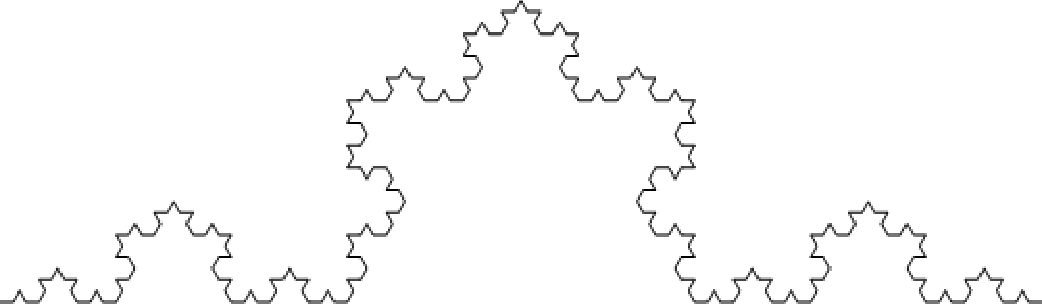
\includegraphics[width=1.0\textwidth]{koch_picture}
\caption{
Let $K_0 \in \RR^2$ be the segment $[0,1]\times \ENCLOSE{0}$,
the figure shows the fourth iterate $K_4 = T^4(K_0)$ of the contraction defining
the K{\"o}ch curve.
On page~\pageref{code:Koch}, the code to generate the figure.
\index{K{\"o}ch curve}%
}
\label{fig:koch}
\end{figure}

\begin{example}[K{\"o}ch curve]
Let $R_\theta\colon \RR^2 \to \RR^2$ be the rotation centered at the origin by
$\theta$ radians counterclockwise. Let $\alpha = \pi/3$, $p=(1,0)$, and let
$\phi_1, \phi_2, \phi_3, \phi_4 \colon \RR^2 \to \RR^2$ be the functions defined
by:
\begin{align*}
\phi_1(v) = \frac{v}{3}, \qquad
\phi_2(v) = R_{\alpha}\frac{v}{3} + \phi_1(p), \\
\phi_3(v) = R_{-\alpha}\frac{v}{3} + \phi_2(p), \qquad
\phi_4(v) = \frac{v}{3} + \phi_3(p).
\end{align*}
Then there exists a unique closed set $K\subset \RR^2$ such that
\[
  K = \phi_1(K) \cup \phi_2(K) \cup \phi_3(K) \cup \phi_4(K).
\]
The set $K$ is called the \emph{K{\"o}ch curve}%
\mymargin{K{\"o}ch curve}%
\index{K{\"o}ch curve}. 
It is a self-similar fractal as it is composed of four scaled copies of itself.
\end{example}